\documentclass[12pt, psamsfonts]{amsart}

%-------Packages---------
\usepackage{amssymb,amsfonts}
\usepackage{fullpage}
\usepackage{todonotes}
\usepackage{physics}
\usepackage[all,arc]{xy}
\usepackage{enumerate}
\usepackage{mathrsfs}
\usepackage{theoremref}
\usepackage{graphicx}
\usepackage[bookmarks]{hyperref}

%--------Theorem Environments--------
%theoremstyle{plain} --- default
\newtheorem{thm}{Theorem}[section]
\newtheorem{cor}[thm]{Corollary}
\newtheorem{prop}[thm]{Proposition}
\newtheorem{lem}[thm]{Lemma}
\newtheorem{conj}[thm]{Conjecture}
\newtheorem{quest}[thm]{Question}

\theoremstyle{definition}
\newtheorem{defn}[thm]{Definition}
\newtheorem{defns}[thm]{Definitions}
\newtheorem{con}[thm]{Construction}
\newtheorem{exmp}[thm]{Example}
\newtheorem{exmps}[thm]{Examples}
\newtheorem{notn}[thm]{Notation}
\newtheorem{notns}[thm]{Notations}
\newtheorem{addm}[thm]{Addendum}
\newtheorem*{exer}{Exercise}

\theoremstyle{remark}
\newtheorem{rem}[thm]{Remark}
\newtheorem{rems}[thm]{Remarks}
\newtheorem{warn}[thm]{Warning}
\newtheorem{sch}[thm]{Scholium}

\DeclareMathOperator{\Hom}{Hom}
\DeclareMathOperator{\Id}{Id}
\DeclareMathOperator{\RP}{\mathbb{R}\mathbf{P}^2}

\makeatletter
\let\c@equation\c@thm
\makeatother
\numberwithin{equation}{section}

\bibliographystyle{plain}

\begin{document}

\title{Math 611 (Due 10/2)}
\author{Hidenori Shinohara}
\maketitle

\begin{exer}{(Problem 10, Chapter 1.3)}
  Find all the connected 2-sheeted and 3-sheeted covering spaces of $S^1 \vee S^1$, up to isomorphisms of covering spaces without base points.
\end{exer}

\begin{proof}
  Let $X = S^1 \vee S^1$.
  By the discussion on P.70 of the textbook, we know that $n$-sheeted covering spaces of $X$ are classified by equivalence classes of homomorphisms $\pi_1(X, x_0) \rightarrow S_n$.
  \begin{figure}
    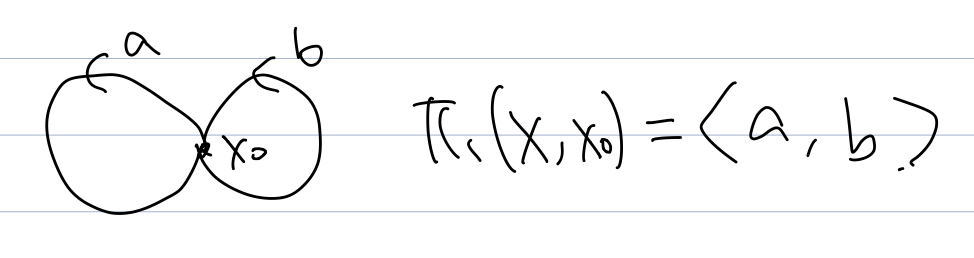
\includegraphics[width=.5\linewidth]{problem10_s1.jpeg}
    \caption{Problem 10 ($X = S^1 \vee S^1$)}
    \label{fig:problem10}
  \end{figure}
  Let $a, b$ denote the paths in $X$ as in Figure \ref{fig:problem10}.
  We can identify each homomorphism $\phi$ by checking what $\phi$ maps $a$ and $b$ to.
  (Strictly speaking, $\pi_1(X, x_0)$ is generated by $[a], [b]$, but we will abuse notations by writing $a$ and $b$ instead of $[a], [b]$.)


  The following are all the cases.
  Figure \ref{fig:problem10_2_sheeted} shows the corresponding graphs.
  \begin{itemize}
    \item
      Case 1: $\phi_1(a) = \phi_1(b) = (1)$.
      The space that corresponds to this homomorphism is disconnected.
    \item
      Case 2: $\phi_2(a) = (12), \phi_2(b) = (1)$.
      This generates a connected covering space.
    \item
      Case 3: $\phi_3(a) = (1), \phi_3(b) = (12)$.
      This generates a connected covering space.
    \item
      Case 4: $\phi_4(a) = (12), \phi_4(b) = (12)$.
      This generates a connected covering space.
  \end{itemize}

  $\phi_2 \not\sim \phi_3, \phi_2 \not\sim \phi_3, \phi_2 \not\sim \phi_3$, which can be verified easily since there are only two elements in $S_2$.
  (For instance, $\phi_2 \ne \phi_3$ and $(12)\phi_2(12) \ne \phi_3$ imply that $\phi_2 \not\sim \phi_3$.)

  Thus the three graphs corresponding to Case 2, 3 and 4 in Figure \ref{fig:problem10_2_sheeted} are all the 2-sheeted covering spaces of $X$.

  \begin{figure}
    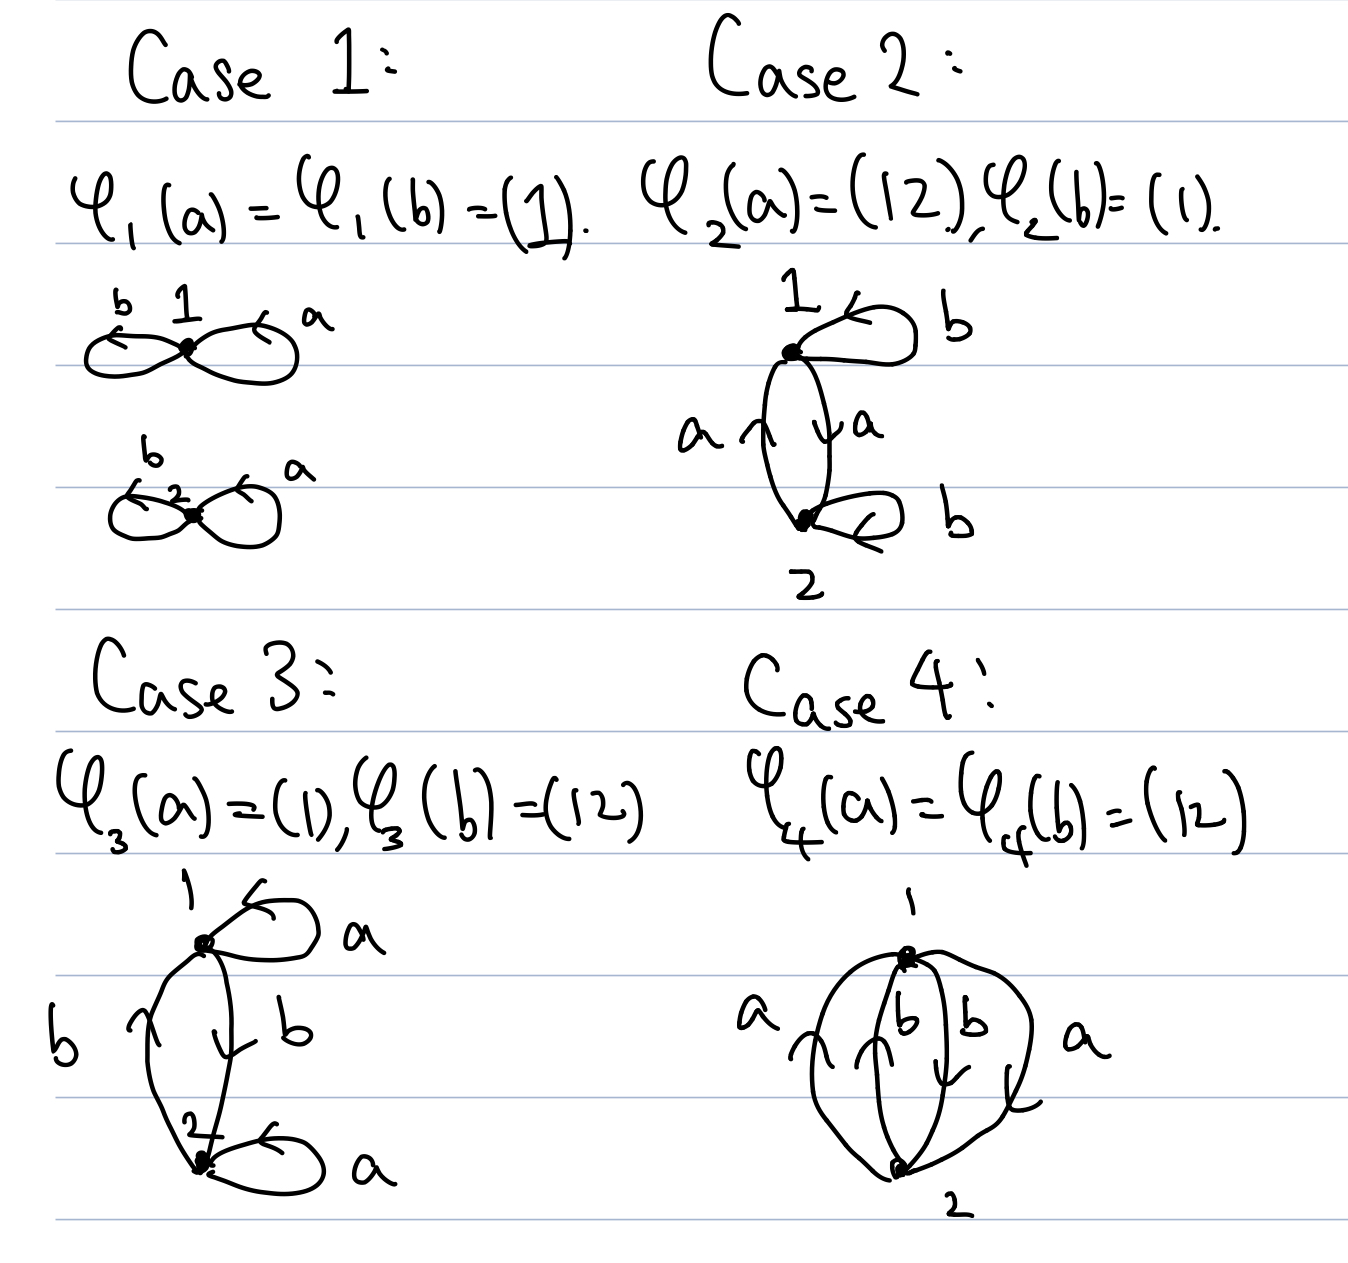
\includegraphics[width=.5\linewidth]{problem10_2_sheeted.jpeg}
    \caption{Problem 10 (2-sheeted covers)}
    \label{fig:problem10_2_sheeted}
  \end{figure}

  We will take the exact same approach for the case of 3.
  If a certain vertex is fixed in both $\phi(a)$ and $\phi(b)$, then such a vertex is disjoint from the rest of the graph.
  We will use that property to reduce the possibilities.
  \begin{figure}
    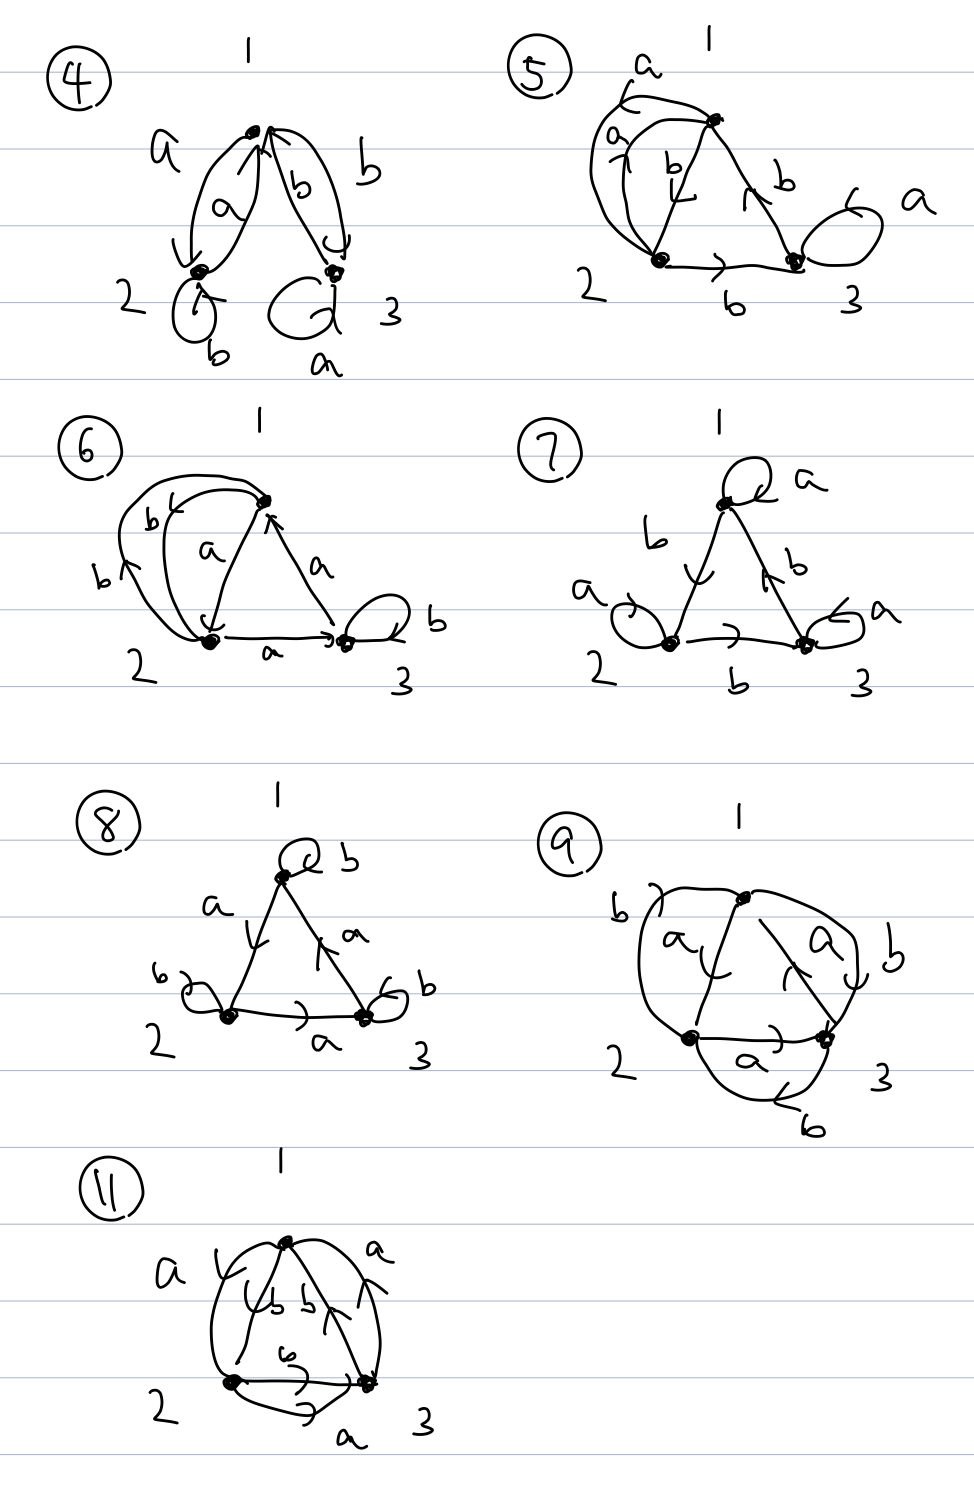
\includegraphics[width=.5\linewidth]{problem10_3_sheeted.jpeg}
    \caption{Problem 10 (3-sheeted)}
    \label{fig:problem10_3_sheeted}
  \end{figure}
  \begin{itemize}
    \item Case 1: $\phi_{1}: a \mapsto (1), b \mapsto (1)$
      The following maps are conjugates of $\phi_{1}$
      \begin{itemize}
        \item $a \mapsto (1), b \mapsto (1)$
      \end{itemize}
      This graph is not connected because every vertex is fixed.
    \item Case 2: $\phi_{2}: a \mapsto (12), b \mapsto (1)$
      The following maps are conjugates of $\phi_{2}$
      \begin{itemize}
        \item $a \mapsto (23), b \mapsto (1)$
        \item $a \mapsto (13), b \mapsto (1)$
        \item $a \mapsto (12), b \mapsto (1)$
      \end{itemize}
      This graph is not connected because vertex 3 is fixed.
    \item Case 3: $\phi_{3}: a \mapsto (1), b \mapsto (12)$
      The following maps are conjugates of $\phi_{3}$
      \begin{itemize}
        \item $a \mapsto (1), b \mapsto (12)$
        \item $a \mapsto (1), b \mapsto (23)$
        \item $a \mapsto (1), b \mapsto (13)$
      \end{itemize}
      This is the same as Case 2.
    \item Case 4: $\phi_{4}: a \mapsto (12), b \mapsto (13)$
      The following maps are conjugates of $\phi_{4}$
      \begin{itemize}
        \item $a \mapsto (13), b \mapsto (12)$
        \item $a \mapsto (12), b \mapsto (23)$
        \item $a \mapsto (12), b \mapsto (13)$
        \item $a \mapsto (13), b \mapsto (23)$
        \item $a \mapsto (23), b \mapsto (12)$
        \item $a \mapsto (23), b \mapsto (13)$
      \end{itemize}
      See Figure \ref{fig:problem10_3_sheeted}.
    \item Case 5: $\phi_{5}: a \mapsto (12), b \mapsto (123)$
      The following maps are conjugates of $\phi_{5}$
      \begin{itemize}
        \item $a \mapsto (23), b \mapsto (123)$
        \item $a \mapsto (12), b \mapsto (123)$
        \item $a \mapsto (12), b \mapsto (132)$
        \item $a \mapsto (13), b \mapsto (132)$
        \item $a \mapsto (13), b \mapsto (123)$
        \item $a \mapsto (23), b \mapsto (132)$
      \end{itemize}
      See Figure \ref{fig:problem10_3_sheeted}.
    \item Case 6: $\phi_{6}: a \mapsto (123), b \mapsto (12)$
      The following maps are conjugates of $\phi_{6}$
      \begin{itemize}
        \item $a \mapsto (123), b \mapsto (13)$
        \item $a \mapsto (132), b \mapsto (12)$
        \item $a \mapsto (132), b \mapsto (23)$
        \item $a \mapsto (132), b \mapsto (13)$
        \item $a \mapsto (123), b \mapsto (12)$
        \item $a \mapsto (123), b \mapsto (23)$
      \end{itemize}
      See Figure \ref{fig:problem10_3_sheeted}.
    \item Case 7: $\phi_{7}: a \mapsto (1), b \mapsto (123)$
      The following maps are conjugates of $\phi_{7}$
      \begin{itemize}
        \item $a \mapsto (1), b \mapsto (132)$
        \item $a \mapsto (1), b \mapsto (123)$
      \end{itemize}
      See Figure \ref{fig:problem10_3_sheeted}.
    \item Case 8: $\phi_{8}: a \mapsto (123), b \mapsto (1)$
      The following maps are conjugates of $\phi_{8}$
      \begin{itemize}
        \item $a \mapsto (132), b \mapsto (1)$
        \item $a \mapsto (123), b \mapsto (1)$
      \end{itemize}
      See Figure \ref{fig:problem10_3_sheeted}.
    \item Case 9: $\phi_{9}: a \mapsto (123), b \mapsto (132)$
      The following maps are conjugates of $\phi_{9}$
      \begin{itemize}
        \item $a \mapsto (123), b \mapsto (132)$
        \item $a \mapsto (132), b \mapsto (123)$
      \end{itemize}
      See Figure \ref{fig:problem10_3_sheeted}.
    \item Case 10: $\phi_{10}: a \mapsto (23), b \mapsto (23)$
      The following maps are conjugates of $\phi_{10}$
      \begin{itemize}
        \item $a \mapsto (12), b \mapsto (12)$
        \item $a \mapsto (23), b \mapsto (23)$
        \item $a \mapsto (13), b \mapsto (13)$
      \end{itemize}
      Vertex 1 is disconnected from the rest of the graph since it is fixed.
    \item Case 11: $\phi_{11}: a \mapsto (123), b \mapsto (123)$
      The following maps are conjugates of $\phi_{11}$
      \begin{itemize}
        \item $a \mapsto (132), b \mapsto (132)$
        \item $a \mapsto (123), b \mapsto (123)$
      \end{itemize}
      See Figure \ref{fig:problem10_3_sheeted}.
  \end{itemize}
  Since there are 6 elements in $S_3$, there are 36 possible homomorphisms.
  The list above contains all of them.
  Therefore, Figure \ref{fig:problem10_3_sheeted} lists all the possible 3-sheeted covers.
\end{proof}

\begin{exer}{(Problem 11, Chapter 1.3)}
  Construct finite graphs $X_1$ and $X_2$ having a common finite-sheeted covering space $\tilde{X}_1 = \tilde{X}_2$, but such that there is no space having both $X_1$ and $X_2$ as covering spaces.
\end{exer}

\begin{proof}
  Figure \ref{fig:problem11} shows $X_1, X_2$ and $\tilde{X}_1 = \tilde{X}_2$.
  \begin{figure}
    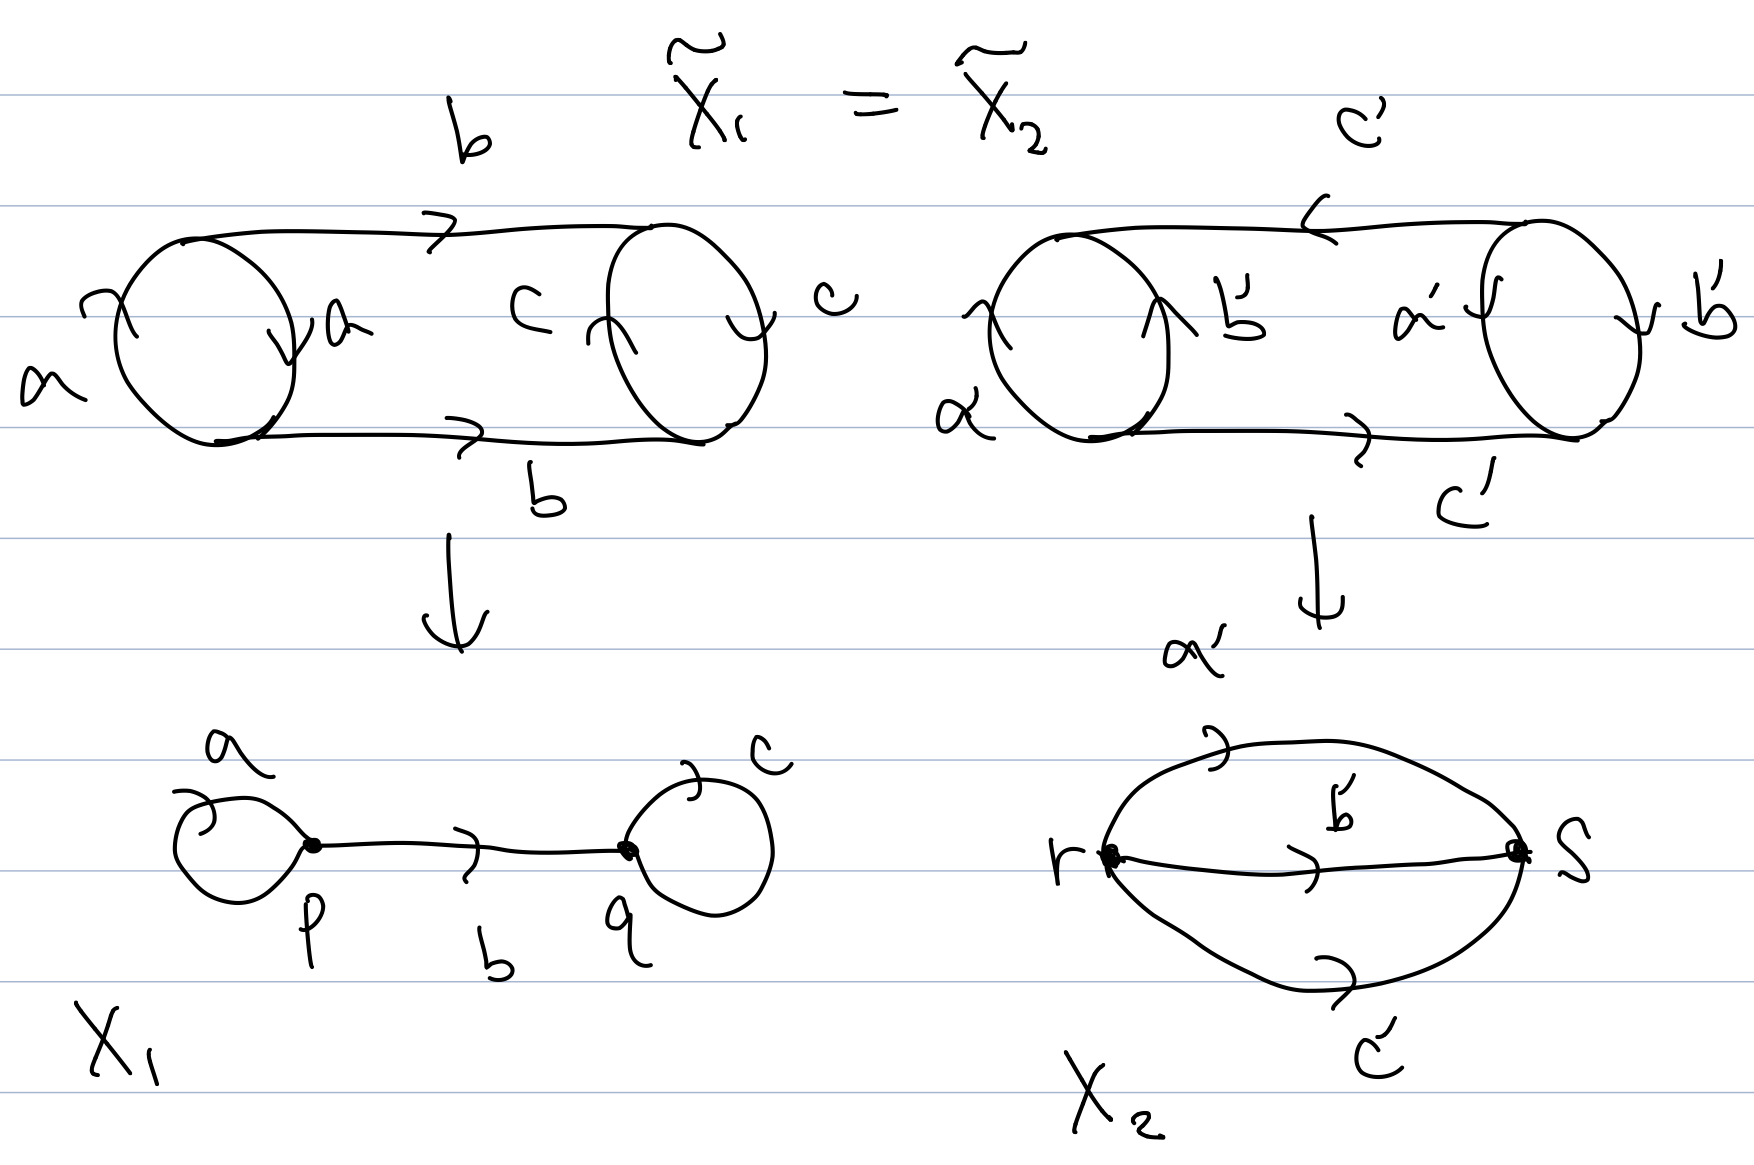
\includegraphics[width=.5\linewidth]{problem11.jpeg}
    \caption{Problem 11}
    \label{fig:problem11}
  \end{figure}
  
  We claim that there exists no space having both $X_1$ and $X_2$ as covering spaces.
  On the contrary, suppose there exists such a space $X$ with covering maps $p_1: X_1 \rightarrow X, p_2: X_2 \rightarrow X$.
  Then every point in $X$ must have a neighborhood that homeomorphic to an open subset of $X_1$.
  Since $X_1$ is a graph, that means $X$ is locally a line and a vertex with edges.
  In other words, $X$ must be a graph.

  There must exist a neighborhood of $p_1(p)$ and a neighborhood of $p$ such that they are homeomorphic.
  Since $p$ is a vertex of degree 3, $p_1(p)$ must be a vertex of degree 3 as well.
  Similarly, $p_1(q)$ must be a vertex of degree 3 as well.

  Since $p, q$ are the only vertices of $X_1$, $X$ contains at most two vertices and their degrees must be 3.
  Since the sum of degrees of all vertices must be even from elementary graph theory, $X$ must contain two vertices of degree 3.

  If $X$ only consists of loops, then the degree of each vertex will be even.
  Thus the two vertices must be joined by at least one edge.
  Then if one vertex has a loop, the other must have a loop as well in order to have degree 3.
  If there exists another edge joining the two vertices, there must be a third one in order for the two vertices to have degree 3.
  Therefore, $X_1, X_2$ are the only graphs with two vertices of degree 3.
  Thus $X = X_1$ or $X = X_2$.

  Suppose that $X_1$ is a covering space of $X_2$ with a covering map $f: X_1 \rightarrow X_2$.
  Without loss of generality, $f(p) = r, f(q) = s$.
  Consider the path $a'$ in $X_2$.
  Lifting $a'$ to $X_1$ will result in a path from $p$ to $q$.
  This implies that $f$ maps points on the path $b$ into points on a path $a'$.
  
  Now consider the path $b'$ in $X_2$.
  Lifting $b'$ to $X_1$ will again result in a path from $p$ to $q$.
  This implies that $f$ maps points on the path $b$ into points on a path $b'$.

  This implies that every point on the path $b$ must be mapped to $r$ or $s$.
  This is a contradiction because $f$ is continuous and $\{ b(t) \mid t \in [0, 1] \}$ is connected, but $f(\{ b(t) \mid t \in [0, 1] \}) = \{ r, s \}$ is disconnected.

  Thus $X_1$ is not a covering space of $X_2$.

  Similarly, suppose that $X_2$ is a covering space of $X_1$ with a covering map $g: X_2 \rightarrow X_1$.
  Without loss of generality, $g(r) = p, g(s) = q$.
  This implies $g^{-1}(p) = \{ r \}$, so the number of sheets is 1.
  In other words, $g$ is injective.
  Consider the path $a$ in $X_1$.
  Lifting $a$ to $X_2$ results into a loop based at $r$.
  Since $a: I \rightarrow X_1$ is injective, $\tilde{a}: I \rightarrow X_2$ is injective since $g \circ \tilde{a} = a$.
  Then $\tilde{a}(t) = s$ for some $t \in [0, 1]$, so $a(t) = g(\tilde{a}(t)) = g(s) = q$.
  However, $q$ is not a point on $a$.
  This is a contradiction, so $X_2$ is not a covering space of $X_1$.

  Hence, there exists no space that has both $X_1$ and $X_2$ as covering spaces.
\end{proof}

\begin{exer}{(Problem 14, Chapter 1.3)}
  Find all the connected covering spaces of $\RP \vee \RP$.
\end{exer}

\begin{proof}
  Let $X = \RP \vee \RP$.
  By Theorem 1.38 of the textbook, it suffices to check all the conjugacy classes of subgroups of $\pi_1(X, x_0)$ and corresponding covering spaces.

  Since $\pi_1(\RP) = \langle a \mid a^2 \rangle$, $G = \pi_1(X) = \langle a, b \mid a^2 = b^2 = e \rangle$ by Van Kampen.

  We will use three properties of elements in $\pi_1(X)$:

  \begin{itemize}
    \item
      Every word can be uniquely expressed as a finite alternating sequence of $a$ and $b$ because $a^2 = b^2 = e$.
    \item
      The parity of the length of a word does not depend on its representation because $a^2 = b^2 = 1$.
      Given two words $x_1 \cdots x_n = y_1 \cdots y_m$ where $x_i, y_j \in \{ a, b \}$, $x_1 \cdots x_n y_m \cdots y_1 = e$.
      Since the order of $a$ and $b$ are both 2, $x_1 \cdots x_n y_m \cdots y_1$ must consist of even numbers of $a$ and $b$.
      Thus $n + m$ is even, so $n \equiv m \pmod 2$.
      This also implies that the parity of the number of $a$ or $b$ in a word is independent of its representation.
    \item
      The parity of the length of a word is invariant under conjugation because conjugating a word appends an even number of letters.
    \item
      The parity of the number of $a$ or $b$ is invariant under conjugation because conjugating a word appends even numbers of $a$ and $b$.
  \end{itemize}

  We will call a subgroup even if the length of each element in it is even, and we will call a subgroup odd otherwise.
  Since the parity of the length of a word is invariant under conjugation, even subgroups and odd subgroups are not conjugates of each other.
  Therefore, we will classify even subgroups and odd subgroups separately.
  \begin{figure}
    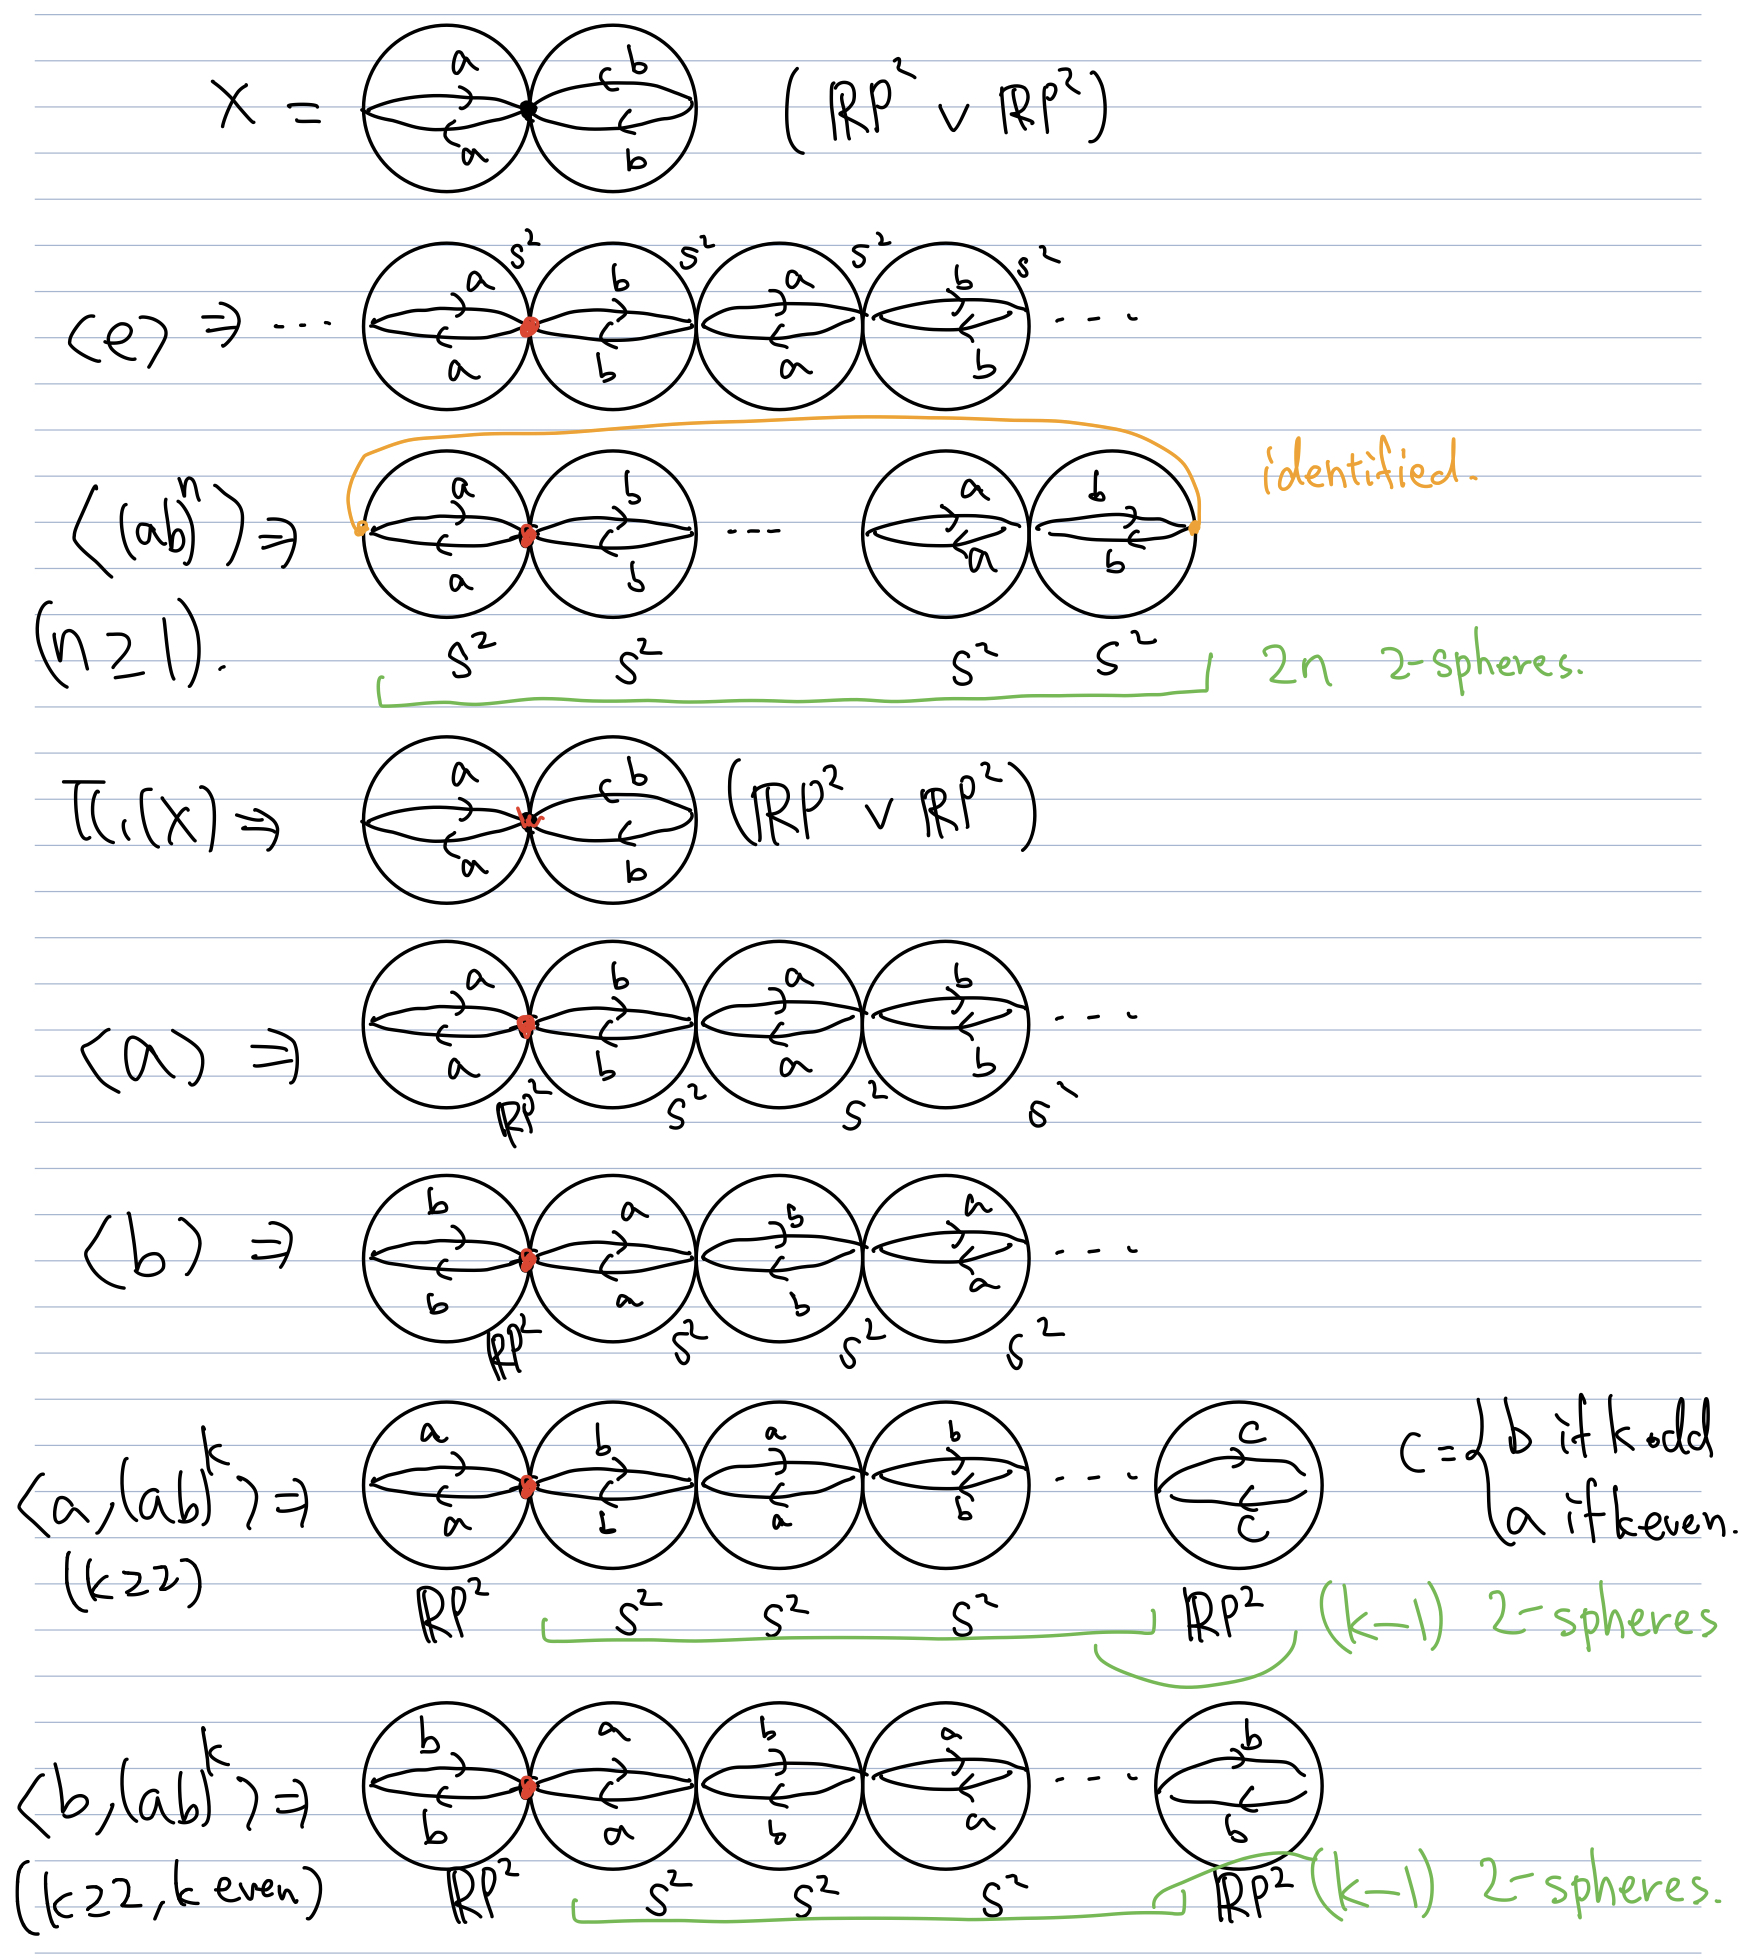
\includegraphics[width=.7\linewidth]{problem14_classification.jpeg}
      \caption{Problem 14}
    \label{fig:problem14}
  \end{figure}

  \begin{itemize}
    \item
      Let $H \subset G$ be an even subgroup.
      Every even length word can be expressed as $(ab)^k$ for some $k \in \mathbb{Z}$.
      Since $(ab)^k = e$ if and only if $k = 0$, this number $k$ is unique to each word of odd length.
      Let $\phi: H \rightarrow \mathbb{Z}$ be defined such that $\phi((ab)^k) = k$.
      Then $\phi(H)$ is a subgroup of $(\mathbb{Z}, +)$.
      Since $\mathbb{Z}$ is an infinite cyclic group, $\phi(H) = (n)$ for some non-negative integer $n$.
      Thus $H = \ev{(ab)^n}$.
      For each $n$, Figure \ref{fig:problem14} shows the covering space corresponding to $\ev{(ab)^n}$.
      Since the number of sheets is the same as the index of the subset by Proposition 1.32 of the textbook, $[\pi_1(X):\ev{(ab)^n}]$ is infinite when $n = 0$ and the index is $2n$ when $n \geq 1$.
      Since the index of a subgroup is invariant under conjugation, $\ev{(ab)^n} \not\sim \ev{(ab)^m}$ whenever $n \ne m, n \geq 0, m \geq 0$.
    \item
      Let $H \subset G$ be an odd subgroup.
      Every odd element is an alternating sequence of $a$ and $b$ which starts and ends with the same letter.
      Thus, every odd element is conjugate to $a$ or $b$.
      Let $w \in H$ be a word of odd length.
      Then $w$ is $xax^{-1}$ or $xbx^{-1}$ for some $x$.
      Then $x^{-1}Hx$ contains $a$ or $b$.
      This implies that every odd subgroup is conjugate to an odd subgroup containing either $a$ or $b$ (possibly both).
      Since we are classifying subgroups up to conjugation, we can assume that $H$ contains $a$ or $b$ without loss of generality.

      We will first assume that $a \in H$ since the argument for the case $b \in H$ will be the same.
      Let $H'$ be a subset of $H$ containing only words of even length.
      Since $e \in H'$ and $xy^{-1}$ is another word of even length for each $x, y \in H'$, $H'$ is a subgroup of $H$.
      Then $H'$ is an even subgroup of $G$, so by the argument above, $H' = \ev{(ab)^n}$ for some $n \geq 0$.

      Let $w \in H$.
      \begin{itemize}
        \item
          If the length of $w$ is even, $w \in H' = \ev{(ab)^n} = \ev{a, (ab)^n}$.
        \item
          If the length of $w$ is odd, $aw \in H' = \ev{(ab)^n} = \ev{a, (ab)^n}$.
          Since $aw \in \ev{a, (ab)^n}$, $w \in \ev{a, (ab)^n}$.
      \end{itemize}
      Therefore, $H = \ev{a, (ab)^n}$.
      
      \begin{itemize}
        \item
          When $n = 0$, $H = \ev{a}$.
        \item
          When $n = 1$, $H = \ev{a, ab} = \ev{a, b} = G$.
        \item
          When $n \geq 2$, $H = \ev{a, (ab)^n}$.
      \end{itemize}

      Using the same argument, if $b \in H$, we can conclude that $H$ is one of the following:
      \begin{itemize}
        \item
          When $n = 0$, $H = \ev{b}$.
        \item
          When $n = 1$, $H = \ev{b, ab} = \ev{a, b} = G$.
        \item
          When $n \geq 2$, $H = \ev{b, (ab)^n}$.
      \end{itemize}

      By putting these together, if $H$ is an odd subgroup, it must be conjugate to one or more of the following:
      \begin{itemize}
        \item
          $\ev{a}$.
        \item
          $\ev{b}$.
        \item
          $\ev{a, (ab)^k}$ where $k \geq 2$.
        \item
          $\ev{b, (ab)^k}$ where $k \geq 2$.
        \item
          $G$.
      \end{itemize}
      It suffices to classify these subgroups up to conjugation since this is an exhaustive list of odd subgroups up to conjugation.

      First, we will use the index of each subgroup to classify them.
      If two subgroups have different indices, they cannot be conjugate to each other.
      By Figure \ref{fig:problem14}, $[G: \ev{a}] = [G: \ev{b}] = \infty$ and $[G: \ev{a, (ab)^k}] = [G: \ev{b, (ab)^k}] = k$ for each $k \geq 2$.
      Moreover, the parity of the number of $b$ in each word of $\ev{a}$ is even since it is always 0.
      On the other hand, the parity of the number of $b$ in $b \in \ev{b}$ is 1.
      Thus $\ev{a}$ and $\ev{b}$ cannot be conjugate to each other.

      Finally, it remains to check if $\ev{a, (ab)^k} \sim \ev{b, (ab)^k}$ for each $k \geq 2$.
      For that purpose, we will consider two cases based on the parity of $k$.
      \begin{itemize}
        \item
          $k \geq 2$ and $k$ is odd.
          Let $k = 2l + 1$.
          \begin{align*}
            \ev{a, (ab)^k}
              &= \ev{a, (ab)^{2l + 1}} \\
              &= \ev{a, (ab)^{l + 1}(ab)^l} \\
              &= \ev{a, (a(ba)^lb)(ab)^l} \\
              &= \ev{a, a(ba)^lb(ab)^l} \\
              &= \ev{a, a(ab)^{-l}b(ab)^l} \\
              &= \ev{a, (ab)^{-l}b(ab)^l} \\
              &\sim \ev{(ab)^la(ab)^{-l}, b} \\
              &= \ev{(ab)^la(ab)^{-l}b, b} \\
              &= \ev{(ab)^{2l + 1}, b} \\
              &= \ev{(ab)^{k}, b}.
          \end{align*}
          Therefore, when $k \geq 2$ and $k$ is odd, $\ev{a, (ab)^k}$ and $\ev{b, (ab)^k}$ are conjugates of each other.
        \item
          $k \geq 2$ and $k$ is even.
          The number of $b$ in $a$ is 0, and the number of $b$ in $(ab)^k$ is $k$.
          In each case, the number of $b$ is even.
          Since every element in $\ev{a, (ab)^k}$ is generated by them, the parity of the number of $b$ in any element of $\ev{a, (ab)^k}$ is even.
          However, the number of $b$ in $b \in \ev{b, (ab)^k}$ is 1, which is odd.
          Therefore, $\ev{a, (ab)^k}$ is not conjugate to $\ev{b, (ab)^k}$.
      \end{itemize}
    \end{itemize}
  Hence, the following is the complete list of all the distinct subgroups of $\pi_1(X)$ up to conjugation and Figure \ref{fig:problem14} has the covering spaces corresponding to each class:
  \begin{itemize}
    \item
      Even subgroups.
      \begin{itemize}
        \item
          $\ev{e}$.
        \item
          $\ev{(ab)^n}$ for $n \geq 1$.
      \end{itemize}
    \item
      Odd subgroups.
      \begin{itemize}
        \item
          $\pi_1(X)$.
        \item
          $\ev{a}$.
        \item
          $\ev{b}$.
        \item
          $\ev{a, (ab)^k}$ for each $k \geq 2$.
        \item
          $\ev{b, (ab)^k}$ for each $k \geq 2$ and $k$ even.
      \end{itemize}
  \end{itemize}
\end{proof}

\end{document}


